%%%%%%%%%%%%%%%%%%%%%%%%%%%%%%%%%%%%%%%%%
% Beamer Presentation
% LaTeX Template
% Version 1.0 (10/11/12)
%
% This template has been downloaded from:
% http://www.LaTeXTemplates.com
%
% License:
% CC BY-NC-SA 3.0 (http://creativecommons.org/licenses/by-nc-sa/3.0/)
%
%%%%%%%%%%%%%%%%%%%%%%%%%%%%%%%%%%%%%%%%% 

%----------------------------------------------------------------------------------------
%   PACKAGES AND THEMES
%----------------------------------------------------------------------------------------

\documentclass[xcolor=dvipsnames]{beamer}
\usepackage{graphicx} % Allows including images
\usepackage{tikz}
\usepackage{pgfplots}
\usepackage{pgf}
\usepackage{soul}
%\usepackage{hyperref}
\pgfplotsset{compat=newest}

%\usepackage{amsmath} % Add amssymb if not using Mathtime
\newcommand\numberthis{\addtocounter{equation}{1}\tag{\theequation}}

% Set arrow type
\input{/Users/mqwilber/Dropbox/Documents/Latex/arrowsnew}
\usetikzlibrary{arrows,shapes,backgrounds}
\tikzset{>=latex}

%\usefonttheme{professionalfonts}
\usepackage{fontspec}
\setsansfont[UprightFont={* Light},
             BoldFont={* SemiBold},
             ItalicFont={* Light Italic},
             BoldItalicFont={* SemiBold Italic}]{Gill Sans}

%\setsansfont[UprightFont={* Light}]{Helvetica}
%\setsansfont{Papyrus}
% \setsansfont[Path = /usr/local/texlive/2014/texmf-dist/fonts/truetype/huerta/alegreya/,
% Extension=.ttf
% ]{AlegreyaSC-Regular}

% Set graphics path
\graphicspath{{images/}}


\renewcommand\footnoterule{}
\newcommand{\tc}{\textcolor{red}}
\newcommand{\tb}{\textcolor{blue}}
\newcommand\ig[1]{\includegraphics[width=#1\textwidth]}

\definecolor{dgreen}{rgb}{0.,0.6,0.}
\setbeamertemplate{caption}{\raggedright\insertcaption\par}
% \usepackage[dvipsnames]{xcolor}

% Color of frame title
\setbeamercolor{frametitle}{fg=Black, bg=White}
\setbeamertemplate{frametitle}[two lines]

% Change color of title
\setbeamercolor{title}{fg=Black, bg=White}

% Change color of enumerated list
\setbeamertemplate{enumerate item}{\color{Black}\insertenumlabel.}

\setbeamertemplate{itemize item}{\color{Black}\tikz[baseline=-0.8ex]\draw[black,fill=black] (0,0) circle (.3ex);}
\setbeamertemplate{itemize subitem}{\color{Black}\tikz[baseline=-0.8ex]\draw[black,fill=black] (0,0) circle (.2ex);}

%% Personal commands

% Define frog
\def\cfrog{\includegraphics[width=0.8cm]{/Users/mqwilber/Repos/completed_projects/empirical_taylor_law/docs/presentation/images/frog_sw}}

\def\cfrognew{\includegraphics[width=.15\textwidth]{/Users/mqwilber/Repos/completed_projects/density_dependent_ipm/docs/presentation/images/cfrog}}
\def\cinfrognew{\includegraphics[width=.15\textwidth]{/Users/mqwilber/Repos/completed_projects/density_dependent_ipm/docs/presentation/images/infected_cfrog}}

\def\border{draw, ultra thick, inner sep=.8}

\newcommand{\numfrog}[1]
{   \begin{tikzpicture}
      \node[opacity=0.5] at (0, 0) (frog) {\includegraphics[width=1.4cm]{/Users/mqwilber/Repos/completed_projects/empirical_taylor_law/docs/presentation/images/frog_sw}};
      \node[inner sep=0.8, draw, fill=white] at (0, 0) {\textcolor{black}{#1}};
    \end{tikzpicture}
}

% Footnote without a marker
\newcommand\blfootnote[1]{%
  \begingroup
  \renewcommand\thefootnote{}\footnote{#1}%
  \addtocounter{footnote}{-1}%
  \endgroup
}

\mode<presentation> {

% The Beamer class comes with a number of default slide themes
% which change the colors and layouts of slides. Below this is a list
% of all the themes, uncomment each in turn to see what they look like.

\usetheme{default}
%\usetheme{AnnArbor}
%\usetheme{Antibes}
%\usetheme{Bergen}
%\usetheme{Berkeley}
%\usetheme{Berlin}
%\usetheme{Boadilla}
%\usetheme{CambridgeUS}
%\usetheme{Copenhagen}
%\usetheme{Darmstadt}
%\usetheme{Dresden}
%\usetheme{Frankfurt}
%\usetheme{Goettingen}
%\usetheme{Hannover}
%\usetheme{Ilmenau}
%\usetheme{JuanLesPins}
%\usetheme{Luebeck}
%\usetheme{Madrid}
%\usetheme{Malmoe}
%\usetheme{Marburg}
%\usetheme{Montpellier}
%\usetheme{PaloAlto}
%\usetheme{Pittsburgh}
%\usetheme{Rochester}
%\usetheme{Singapore}
%\usetheme{Szeged}
%\usetheme{Warsaw}

% As well as themes, the Beamer class has a number of color themes
% for any slide theme. Uncomment each of these in turn to see how it
% changes the colors of your current slide theme.

%\usecolortheme{albatross}
%\usecolortheme{beaver}
%\usecolortheme{beetle}
%\usecolortheme{crane}
%\usecolortheme{dolphin}
%\usecolortheme{dove}
%\usecolortheme{fly}
%\usecolortheme{lily}
%\usecolortheme{orchid}
%\usecolortheme{rose}
%\usecolortheme{seagull}
%\usecolortheme{seahorse}
%\usecolortheme{whale}
%\usecolortheme{wolverine}

\setbeamertemplate{footline} % To remove the footer line in all slides uncomment this line
%\setbeamertemplate{footline}[page number] % To replace the footer line in all slides with a simple slide count uncomment this line

\setbeamertemplate{navigation symbols}{} % To remove the navigation symbols from the bottom of all slides uncomment this line
}


% Centers the frametitles of each slide
% \setbeameroption{show notes}
\setbeamertemplate{frametitle}[default][center]

% Adding

\title{RSF and pig movement update} % The
% short
% title appears at the bottom
% of every
% slide, the full title is only on the title page

\author{Lab meeting}
\institute[CSU]
{
\smallskip

}
\date{April 23, 2018} % Date, can be changed to a custom date

%\titlegraphic{\includegraphics[scale=0.25]{example_tpl.png}}

\begin{document}

% Remember pictures
\tikzstyle{every picture}+=[remember picture]
\tikzstyle{na} = [baseline=-.5ex]

% \begin{frame}
% \titlepage % Print the title page as the first slide
% \end{frame}


%------------------------------------------------

\begin{frame}[t]
\frametitle{\underline{Discussion points for today}}
  
  \begin{itemize}
    \item Covariate discussion
    \begin{itemize}
      \item Defining available crop
      \item Defining a ``crop-user''
      \item Defining a crop season
    \end{itemize}
    \item Quantitative cross-population comparison suggestions
  \end{itemize}

\end{frame}

%------------------------------------------------

\begin{frame}[t]
\frametitle{\underline{Overall questions}}

  \begin{enumerate}
    \item Do pigs that use crops use non-crop resources differently than pigs that don't use crops?
    \item Is there evidence that pigs use crops in different ways? 
      \begin{itemize}
        \item e.g. Do pigs move differently once they are in crops and how?
      \end{itemize}
  \end{enumerate} 

  \centering
  \bigskip
  \ig{0.45}{images/cropdamage.pdf}

\end{frame}

%------------------------------------------------

\begin{frame}[t]
\frametitle{\underline{Pig data and covariates}}

  \textbf{Processed pig data}

  \begin{itemize}
    \item 227 pigs, 12 studies
  \end{itemize}

  \bigskip

  \textbf{Covariate data}


  \begin{columns}
    \begin{column}{0.5\textwidth}

      \begin{itemize}
        \item Dist-to-nearest perennial water
        \item Tree cover density
        \item Elevation
        \item Human development index
        \item \textbf{Distance-to-nearest crop}
      \end{itemize}
       
    \end{column}
    \begin{column}{0.5\textwidth}

      \begin{itemize}
        \item NDVI/EVI
        \item Masting tree density
        \item Temperature
        \item Precipitation
        \item Snow depth
      \end{itemize}
    
    \end{column}
  \end{columns}

  \only<2>{

  \bigskip
  How do you define available crop? Distance to nearest crop that has been used previously?}


\end{frame}

%------------------------------------------------

\begin{frame}[t]
\frametitle{\underline{What we are doing is...}}

  \begin{enumerate}
    \item Estimating resource utilization functions for each pig using GPS movement data
    \item Comparing resource utilization between crop and non-crop using pigs
  \end{enumerate}

\end{frame}

%------------------------------------------------

\begin{frame}[t]
\frametitle{\underline{Predicting resource utilization}}
  
  Covariates + movement model $\rightarrow$ prediction of resource utilization

  \begin{enumerate}
    \item \emph{Location-based covariates}: How long a pig remains in a cell as a function of resource

    \item \emph{Directional covariates}: The direction in which a pig moves from that cell as a function of the resource gradient
  \end{enumerate} 

  \bigskip
  \centering
  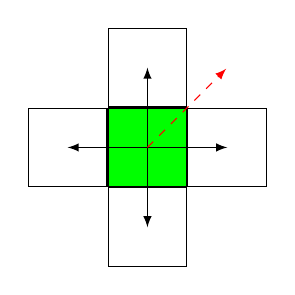
\begin{tikzpicture}
    \node[draw, minimum height=1cm, minimum width=1cm, fill=green] at (0,  0) (mid) {};
    \node[at=(mid.south), below, draw, minimum height=1cm, minimum width=1cm] (down) {};
    \node[at=(mid.north), above, draw, minimum height=1cm, minimum width=1cm] (up) {};
    \node[at=(mid.east), right, draw, minimum height=1cm, minimum width=1cm] (right) {};
    \node[at=(mid.west), left, draw, minimum height=1cm, minimum width=1cm] (left) {};

    \only<2->{
    \draw[->] (mid.center)--(down.center);
    \draw[->] (mid.center)--(up.center);
    \draw[->] (mid.center)--(right.center);
    \draw[->] (mid.center)--(left.center);


    \draw[->, dashed, red] (mid.center)--(1, 1);}
  \end{tikzpicture}

\end{frame}

% ------------------------------------------------

\begin{frame}[t]
\frametitle{\underline{An example from Tejon}}

  \only<1>{\ig{1}{tejonlayers.pdf}}
  \only<2>{\ig{1}{tejonlayers_wpig.pdf}}

\end{frame}

% ------------------------------------------------

\begin{frame}[t]
\frametitle{\underline{Predicted time-invariant resource utilization}}

  \only<1>{
    Assume resource use is constant across day and season (obviously false, but an illustrative place to start)
  }
  
  \only<2>{

  \centering
  \ig{1}{images/canopy.pdf}

  M302 moves significantly slower in increased canopy cover

  }

  \only<3>{

    \centering
    \ig{1}{images/water.pdf}

    M302 moves toward water

  }

  \only<4>{

    \centering
    \ig{1}{images/fruit.pdf}

    M302 moves slower in crops, turns more, but only weakly moves toward crops...not accounting for daily patterns of resource use.

  }

\end{frame}

%------------------------------------------------

\begin{frame}[t]
\frametitle{\underline{Predicted time-variant resource utilization}}
  
  \centering

  \only<1>{
    Allow the use of particular resource to vary with the time of day and season

    \bigskip
    \textbf{Time of day}

    \begin{itemize}
      \item Morning: 1:00-8:00
      \item Midday: 9:00-16:00
      \item Evening: 17:00-0:00 
    \end{itemize}

    \textbf{Season}

    \begin{itemize}
      \item Spring: March, April, May
      \item Summer: June, July, August
      \item Fall: September, October, November
      \item Winter: December, January, February
    \end{itemize}
  }

  \only<2>{
    \ig{1}{images/base.pdf}

    M302 moves slower during midday than the evening or morning
  }

  \only<3>{
    \ig{1}{images/crw.pdf}

    M302 shows more directional movement in the evening and the morning
  }

  \only<4>{
    \ig{1}{images/fruit2.pdf}

    M302 moves toward fruit and nuts in the evening and away in the morning
  }

  \only<5>{
    \ig{1}{images/fruit3.pdf}

    Consistent affect of fruit and nuts in the fall and summer
  }

\end{frame}

%------------------------------------------------

\begin{frame}[t]
\frametitle{\underline{Resource-use and crop-use across studies}}
  
  \centering

  \only<1>{
    \ig{0.9}{cropusers.pdf}
  }

  \only<2>{
    \ig{0.9}{/Users/mqwilber/Repos/rsf_swine/results/crop_use_overall.pdf}
  }

  \only<3>{
    \ig{0.9}{/Users/mqwilber/Repos/rsf_swine/results/crop_use_by_study.pdf}
  }

  % Does the use of non-crop resources distinguish between movement patterns of crop-using and non-cropusing pigs?

\end{frame}

%------------------------------------------------

\begin{frame}[t]
\frametitle{\underline{Question 1: Crop-users vs. non crop-users}}
  
  \centering

  \only<1-2>{
  Does the use of non-crop resources distinguish between movement patterns of crop-using and non-crop-using pigs?}

  \only<2>{
    \bigskip
    \textbf{Yes, but in different ways across studies.}
  }

  \only<3>{
    \ig{0.8}{canopycover_pop.pdf}

    One of the few consistent effects across pigs and studies
  }

  \only<4>{

    \bigskip
    \ig{1}{rf_results.pdf}

    After accounting for crop use, general turning angle and movement speed distinguishes crop-users from non crop-users \emph{in some studies}

  }

  \only<5>{

    \bigskip
    \ig{0.8}{florida_crw.pdf}

    Increased directional movement in florida crop users in morning and evening

  }

  \only<6>{

    \bigskip
    \ig{0.8}{txcamp_crw.pdf}
  }

  \only<7>{

    \bigskip
    \ig{0.8}{srel_contact_crw.pdf}

  }


\end{frame}

%------------------------------------------------

\begin{frame}[t]
\frametitle{\underline{Question 2: Grouping crop users}}
  
  \centering 
  \only<1-2>{
    Do pigs use crops in different ways?  If so, how?
  }

  \bigskip
  \only<2>{\textit{Use a cluster analysis to identify whether there is evidence that pigs differ in the way in which they use crops}}

  \only<3>{
    \centering
    \ig{0.8}{bic.pdf}

    Every study suggests that crop users can be broken into at least 2 groups
  }

  \only<4>{
    \ig{0.9}{srel_contact_groups.pdf}
  }

  \only<5-6>{
    \ig{0.9}{tx_tyler_k1_groups.pdf}
  }

  \only<6>{
    \centering
    Movement patterns within crops describe the primary variation in these groupings
  }

  \only<7>{
    \ig{1}{srel_contact_groups_vector.pdf}
  }

  \only<8>{
    \ig{1}{tx_tyler_k1_groups_vector.pdf}
  }

\end{frame}

%------------------------------------------------

\begin{frame}[t]
\frametitle{\underline{Quantitative cross-population comparison?}}
  
  \begin{itemize}
    \item Differences in seasons and crop type make this challenging
      \begin{itemize}
        \item Suggestions? 
      \end{itemize}
    \item Can still see some interesting patterns with qualitative comparisons
  \end{itemize}
\end{frame}

\end{document}

